\chapter{Feature Selection} \label{chap:selection}

Recall that each feature tells
us something about a training example. Ideally, it should also help us
classify the example. However, in practice and particularly
in medicine, a large number of attributes about a patient is usually recorded,
not all of which are relevant in predicting the class.
Having such a large number of features
is detrimental for two reasons: the training time is significantly
increased because the classifier must incorporate more information than it
needs to, and
this irrelevant information tends to degrade the performance
of even state-of-the-art classifiers such as C4.5 decision trees
\cite{Witten2005}. Clearly, there is an advantage in considering only a subset
of the most relevant features; to find them, we will use what is called
\textit{feature selection}.

Our data set contains 78 features aside from the class, which is a fairly high
number. Many of these attributes
are derived from others in the set: for example, whether or not a patient is
over 65 years of age (the \texttt{age65} feature) is directly dependent on the
value of their \texttt{age} attribute.

\section{Preliminary Removal of Features}
We began the process of feature selection by removing attributes that were
not available upon admission, as these tended to be highly related to the
\texttt{los48} outcome and were a consequence, not a predictor, of LOS. Had
we not removed these features, they would be selected by the feature selection
methods described below due to their high association with \texttt{los48}, but
would actually tell us nothing about what causes a patient to require a
hospital stay of more or less than 2 days.
These attributes were: \texttt{iculos}, \texttt{outcome},
\texttt{disp from ed}, \texttt{disp from hosp}, \texttt{died}, \texttt{rehab},
\texttt{los} and \texttt{eddc}.
The \texttt{id} attribute was also removed because it
simply numbered each record and
indicated nothing about the patient. This left us with 69 attributes.

We then removed 10 other features which were directly derived from others in
the data set: \texttt{gcs1}, \texttt{iss8}, \texttt{mechanism}, \texttt{male},
\texttt{age65}, \texttt{bp1}, \texttt{pr1}, \texttt{rr1}, \texttt{fall} and
\texttt{comorbidity}. At this stage there were 59 features -- still a large
number.

After eliminating redundant or inapplicable features as detailed above, we
considered four \textit{automatic} (correlation-based
feature selection, Pearson correlation, 1R and wrapper selection
using C4.5) and two \textit{manual} feature selection methods (domain expert
selection and the feature set used in existing work on trauma LOS prediction).
These methods are described in the following sections.

\section{Automatic Methods}
Automatic feature selection methods are useful for when we do not have a deep
understanding of the underlying domain and what each attribute really means to
the class. Even if we are well-versed in the domain, evaluating a few different
methods of automatic feature selection can give us new insight into the
learning problem at hand. Here we will describe a few of the methods we used.

\subsection{Correlation-based Feature Selection}
Correlation-based feature selection (CFS) is a method developed by Hall
\cite{Hall2000} which looks for a subset of features that have high correlation
with the class but low intercorrelation among the features. In this case,
correlation between two features is measured using what is called the
\textit{symmetric uncertainty}:
\begin{equation*}
U(A,B) = 2\dfrac{H(A)+H(B)-H(A,B)}{H(A)+H(B)}
\end{equation*}
where $A$ and $B$ are two nominal attributes and $H$ is the entropy function
denoted by Equation \ref{eqn:entropy} in Chapter \ref{chap:classification}.
The entropies are calculated from the probabilities of each feature value, and
$H(A,B)$, the joint entropy of $A$ and $B$, is calculated from the
probabilities of each combination of values of $A$ and $B$. Note that $U(A,B)$
is always between 0 and 1.

To evaluate the ``goodness'' of a subset of features with the class $C$, we
compute:
\begin{equation}
\label{eqn:cfs}
\dfrac{\sum_j U(A_j,C)}{\sqrt{\sum_i \sum_j U(A_i,A_j)}}
\end{equation}
where $i$ and $j$ range over the features in the subset being evaluated. The
maximum value that Equation \ref{eqn:cfs} can obtain is 1 when all features
correlate perfectly with the class and also with each other -- the numerator
becomes $n$ and the denominator $\sqrt{n^2}$ if the subset has $n$ features.

\subsection{Pearson Correlation Coefficient}
The Pearson correlation coefficient measures the degree of linear correlation
between two variables. It is always in the range $[-1,1]$, where -1 is total
negative correlation, 0 is no (linear) correlation, and 1 is total positive
correlation. We compute the Pearson correlation between each feature and the
class using:
\begin{equation*}
r_i = \dfrac{\sum_{i=1}^m (x_i-\bar{x})(c-\bar{c})}{\sqrt{(\sum_{i=1}^m x_i-\bar{x})(\sum_{i=1}^m c-\bar{c})}}
\end{equation*}
where $m$ is the number of training examples, $x_i$ is the value of feature
$i$, and $\bar{x}$ and $\bar{c}$ are the arithmetic averages of the feature
values and the class values respectively. (Recall that we also used this
in Chapter \ref{chap:classification} to rank features for use in Ranked
Distance nearest neighbours.) 

A higher value for $r_i$ indicates higher correlation with the class. We
rank all features according to their $r_i$ from highest to lowest, and select
some subset of these either by selecting a fixed number, or selecting all
features that have a correlation above a specified threshold.

\subsection{Information Gain}
Recall from our discussion of decision trees in in Section \ref{sec:c45} that
the information gain (IG) is used to decide which attribute to split on at each
step of the tree. We can also measure the IG of each feature as follows.
If we have a class $C$ and a feature $F$, the entropy of the
class before and after observing the feature is:
\begin{equation*}
\begin{aligned}
& \mathrm{entropy}(C) = - \sum_{c \in C} p(c) \mathrm{log}_2 p(c) \\
& \mathrm{entropy}(C|F) = - \sum_{f \in F} p(f) \sum_{c \in C} p(c|f) \mathrm{log}_2 p(c|f)
\end{aligned}
\end{equation*}
The decrease in entropy reflects the gain in information provided by the
feature and is given by:
\begin{equation*}
IG(C|F) = \mathrm{entropy}(C) - \mathrm{entropy}(C|F)
\end{equation*}

We can compute the IG for each feature and then select subsets of features that
are greater than some threshold we specify.

\subsection{1R}
Another way to evaluate the relevance of features is to use the idea behind the
1R classifier described in Section \ref{sec:zeror}. Recall that the 1R
classifier constructs simple 1-rules based on each feature and uses the feature
that produces the lowest error rate (that is, the highest accuracy) on the data
set to classify unseen examples. These accuracy rates can be calculated for
each feature, which are then used to rank the features from highest to lowest
accuracy. The worst accuracy for any feature is the 0R accuracy, which is the
proportion of the majority class in the data set. This is because if 1R finds
that the accuracy of the rule constructed using a feature is worse than 0R,
then it will not use that rule and predict the majority class instead.

We can also select a fixed number of features or all features above a certain
1R accuracy threshold.

\subsection{Wrapper-based Feature Selection}
The feature selection methods described above (CFS, Pearson correlation and
1R) have been described as \textit{filter} approaches to attribute selection.
Kohavi and John proposed another approach, the \textit{wrapper} approach:
instead of performing feature selection independently of the learning
algorithm using some measure of ``relevance'',
the learning algorithm itself is used to evaluate the goodness of
subsets of features \cite{Kohavi1997}. The difference between the filter
and wrapper approaches is depicted in Figure \ref{fig:wrapper}.

\begin{figure}[h]
\centering
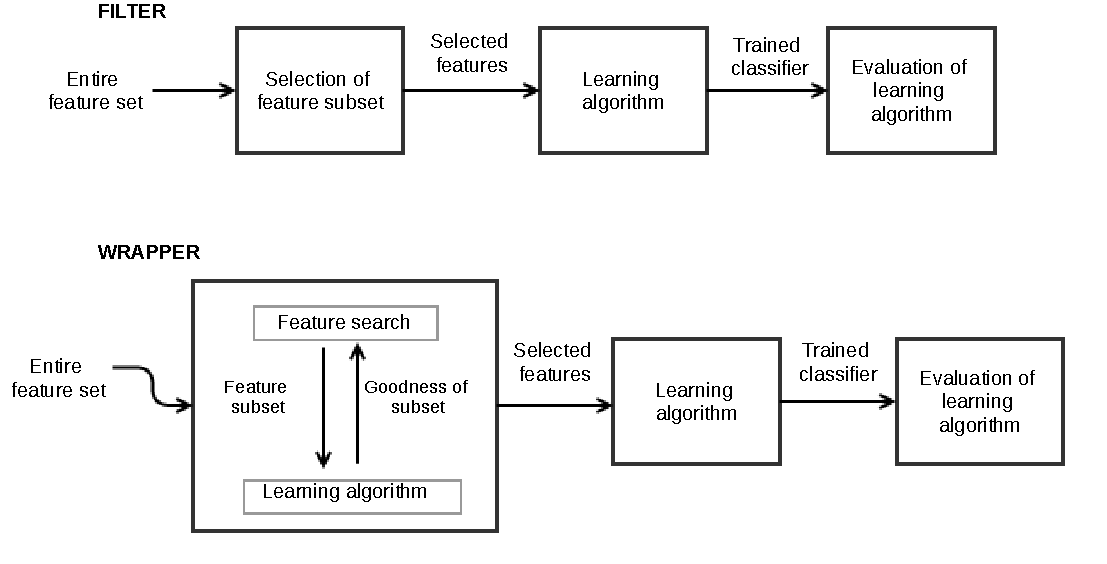
\includegraphics[scale=0.9]{images/method/feature-selection.pdf}
\caption{Filter and wrapper approaches to feature selection. Note the role of
the learning algorithm in the wrapper method.}
\label{fig:wrapper}
\end{figure}

A key advantage of the wrapper approach is that the selected feature sets are
specifically tailored to a learning algorithm, which ensures the best
performance of that algorithm given the data set. However, wrapper approaches
can also be prohibitively slow if the data or feature sets are large and the
chosen learning algorithm expensive to train (such as support vector machines
and multi-layer perceptrons). We will evaluate the use of C4.5 decision trees
(see Section \ref{sec:c45}) in selecting features using the wrapper approach.
Using decision trees to select features is relatively fast as due to the
divide and conquer nature of the learning algorithm, and the tendency of the
trees to select fewer features for learning than other algorithms.

\section{Manual Selection}
\label{sec:manual}
All of the above automatic feature selection methods use some notion of
``relevance'', such as symmetric uncertainty and linear correlation,
in order to determine the best subset of features to select.
Depending on the problem at hand, these definitions of relevance may or may
not work well with the data. In the LOS prediction literature, studies
have enlisted the help of medical domain experts to assist in feature
selection, due to their experience and understanding of the underlying
problem and the effect of the features on the outcome. It will therefore be
worthwhile to compare the performance of classifiers using features selected
automatically and manually.

\subsection{Baseline Feature Set}
The key previous work on trauma LOS prediction was by Dinh et. al.
\cite{Dinh2013a}, who used a specific feature set from the data set that we
use. We would like to use the features they selected as a baseline for
evaluating the other feature selection methods we describe.

\subsection{Domain Expert Selection}
Consultation with a domain expert yielded another feature set that we could
use to compare with the baseline and with the other automatic methods.

\section{Summary}
In this chapter we covered feature selection, which is concerned with reducing
the number of attributes that a learning algorithm needs to consider when
trying to learn a relationship between the training examples and their labels.
We described how we removed redundant and meaningless features before the
feature selection step, and discussed the automatic and manual feature
selection methods we use in our work. The value in using several methods of
each type of feature selection is two-fold: it allows us to not only compare
the performance of the methods, but also to compare the performance of the
different classifiers we use independently of the feature selection method.
